\documentclass[10pt,a4paper,twocolumn,twoside]{article}
\usepackage[utf8]{inputenc}
\usepackage[english]{babel}
\usepackage{graphicx}
\usepackage{fancyhdr}
\usepackage{times}
\usepackage{titlesec}
\usepackage{multirow}
\usepackage{lettrine}
\usepackage[top=2cm, bottom=1.5cm, left=2cm, right=2cm]{geometry}
\usepackage[figurename=Fig.,tablename=TAULA]{caption}
\usepackage{listings, ../common/listings-rust}
\usepackage[hyphens]{url}
\usepackage{hyperref}

\graphicspath{ {img/} }

\lstnewenvironment{code}[1][]%
{
    \scriptsize
    \noindent
    \minipage{\linewidth} 
    \vspace{0.5\baselineskip}
    \lstset{language=Rust, style=colouredRust,#1}}
{\endminipage}

\author{\LARGE\sffamily Josep Maria Domingo Catafal}
\title{\Huge{\sffamily  Design and implementation of a programming language with LLVM }}
\date{}

\newcommand\blfootnote[1]{%
  \begingroup
  \renewcommand\thefootnote{}\footnote{#1}%
  \addtocounter{footnote}{-1}%
  \endgroup
}

\titleformat{\section}
{\large\sffamily\scshape\bfseries}
{\textbf{\thesection}}{1em}{}

\begin{document}

\fancyhead[LO]{\scriptsize AUTOR: TÍTOL DEL TREBALL}
\fancyhead[RO]{\thepage}
\fancyhead[LE]{\thepage}
\fancyhead[RE]{\scriptsize EE/UAB TFG INFORMÀTICA: Design and implementation of a programming language with LLVM}

\fancyfoot[CO,CE]{}

\fancypagestyle{primerapagina}
{
   \fancyhf{}
   \fancyhead[L]{\scriptsize BACHELOR'S THESIS IN COMPUTER SCIENCE, ESCOLA D'ENGINYERIA (EE), UNIVERSITAT AUTÒNOMA DE BARCELONA (UAB)}
   \fancyfoot[C]{\scriptsize Febrer de 2023, Escola d'Enginyeria (UAB)}
}

\renewcommand{\headrulewidth}{0pt}
\renewcommand{\footrulewidth}{0pt}
\pagestyle{fancy}

\twocolumn[\begin{@twocolumnfalse}

\maketitle

\thispagestyle{primerapagina}

\begin{center}
\parbox{0.915\textwidth}
{\sffamily

    \textbf{Abstract--} This thesis presents the design and development of a new
    programming language called \textit{Craft}, using Rust and LLVM. The goal of
    the project is to gain a deeper understanding of how compilers work by
    creating one from scratch using these tools. The language is designed to be
    simple and easy to understand, but at the same time, it aims to be fast and
    efficient, so some sacrifices have to be made. The thesis covers the design
    and implementation of the language, including the lexer, parser, and code
    generation. The project also includes a discussion of the challenges
    encountered during development and suggestions for future work. Overall, the
    project serves as a valuable learning experience for understanding the inner
    workings of compilers and the capabilities of Rust and LLVM.

    \bigskip

    \textbf{Keywords-- } Programming Language, LLVM, SSA, Strongly Typed, Compiled

    \bigskip

    \textbf{Resum--} Aquesta tesi presenta el disseny i desenvolupament d'un nou
    llenguatge de programació anomenat \textit{Craft}, utilitzant Rust i LLVM.
    L'objectiu del projecte és aconseguir una comprensió més profunda de com
    funcionen els compiladors creant-ne un des de zero amb aquestes eines. El
    llenguatge està dissenyat per ser senzill i fàcil d'entendre, però al mateix
    temps, pretén ser ràpid i eficient, per la qual cosa s'han de fer alguns
    sacrificis. La tesi cobreix el disseny i la implementació del llenguatge,
    incloent-hi el lexer, el parser i la generació de codi. El projecte també
    inclou una discussió sobre els reptes trobats durant el desenvolupament i
    suggeriments per a treballs futurs. En general, el projecte serveix com una
    valuosa experiència d'aprenentatge per comprendre el funcionament intern
    dels compiladors i les capacitats de Rust i LLVM.

    \bigskip

    \textbf{Paraules clau-- } Llenguatge de programació, LLVM, SSA, Fortament tipat, Compilat
}
\end{center}

\bigskip
\end{@twocolumnfalse}]

\blfootnote{$\bullet$ E-mail de contacte: jdomingocatafal@gmail.com}
\blfootnote{$\bullet$ Menció realitzada: Computació}
\blfootnote{$\bullet$ Treball tutoritzat per: Javier Sanchez Pujadas (Ciències de la Computació)}
\blfootnote{$\bullet$ Curs 2022/23}

\section{Introduction} \lettrine[lines=3]{H}{istorically}, there has always been
a dilemma between the speed of execution, and speed of development. Some
languages are easy to program: they allow the programmer to not worry about
low-level concepts such as memory management, and create abstractions that
streamline the development. The problem is that these abstractions limit the
language's efficiency, and create slower programs. Another reason that allows
speeding up the development is dynamic typing, as it frees the user from the
mental overhead that comes with deciding the type that should be used. But this
comes with its own disadvantages, since it is very likely that you will
encounter runtime errors unless you use something like a static analyzer. These
languages tend to be interpreted in order to save the programmer the time it
takes to recompile the program, but it has an impact on the runtime
performance of the program if we compare it to compiled languages. Python, for
example, would be one of the largest representatives of this group of languages.
On the other hand we have languages like C, which have almost no abstraction and
the programmer must be aware of what he is doing in every line of code he
writes. They are languages that provide very good performance, but slow down the
development, as the programmer must take into account many low-level concepts.
An additional problem is that when managing memory manually, it opens the door
to a lot of runtime errors in the form of memory leaks and segmentation faults.
Currently, there are languages like Rust that solve these memory management
issues without losing performance, but the development is still slow (maybe even
slower) and the compilation time long. These languages tend to be strongly
typed, which helps reduces runtime errors.

In this thesis we will explore the different types of programming languages, and
we will implement a simple programming language that aims to find balance 
between the different trade-offs we talked about.

\section{State of the art}
A programming language resembles, in a way, a natural language, and like natural
languages, there's a lot of different ones with different properties. We mainly
have two different ways to classify them: by paradigm and by how they are
implemented. The paradigm allows us to classify based on their features and the
way we write programs with them. It tells us something about the design of the
language. On the other hand we have the implementation which tells us
information about how the programs are run. About how the code we write turns
into instructions the CPU can execute. A programming language can have many
implementations, but there's usually one that is the "official" one, and that's
the ones we are going to focus on.

\subsection{Paradigms}
In the following sections we are going to take a look at the main paradigms in
programming languages, even though, some of them may be considered sub-paradigms
of the others. It's also important to note that most programming languages can
fit into multiple of these paradigms, and thus they are multi-paradigm. We are
going to discuss the most popular paradigms, but there are many more.

\subsubsection{Imperative}
Imperative programming languages follow a model of programming that is based on
statements that change the state of the program. When we write an imperative 
program, we specify step by step what the computer has to do. Imperative 
programming is often implemented as procedural programming, a subtype in which
statements are structured into procedures (also known as functions). Most of
the programming languages we use nowadays can fit into this category, including
C/C++, Java, C\#, Go, Lua, JavaScript, etc.

\subsubsection{Object-oriented}
It's a subtype of imperative and procedural programming, in which data and
behavior is grouped in units called objects. These objects hold data, and they
can be modified by functions known as methods. The main representatives of this
paradigm are languages like Java, C\# or C++. These languages represent objects
using classes and have many abstractions like inheritance and polymorphism.

\subsubsection{Functional}
Functional programming has the idea of treating computation as the evaluation of
mathematical functions. Most of the functional languages are characterized by
the use of recursive functions, immutable data and anonymous functions. Even
though most modern languages incorporate functional programming in one way or
another, some languages that we could call functional are Haskell (being one of
the purest), OCaml, Clojure, Scala or Lisp, between others.

\subsubsection{Logic}
Logic programming is a programming paradigm that is based on formal logic. Their
reasoning is similar to the SQL database language. Some examples of logic
programming languages include Prolog or Datalog.

\subsubsection{Scripting}
Scripting languages are languages that are aimed to writing scripts and small
programs that try to solve a very specific problem, like automating a task. They
are also embedded in other programs, to allow the user to add or modify
functionality of it by writing scripts. Some popular scripting languages are 
Python, Lua and command languages like Bash or Fish.

\subsection{Implementations}
There are different ways to implement a programming language. One is by writing
a compiler and the other one is by writing an interpreter. Both have it's
upsides and it's downsides, and usually, depending on the design of the
programming language and its goals, one may be a better option than the other.

\subsubsection{Interpreted}
Interpreted languages, are languages that don't need to be compiled before they
are run. When you run a program they take the original source code and interpret
it at runtime. The major downside of this type of implementations is that we may
have made an error writing the code, and we won't find out until we run it. This
can be quite dangerous since it means the program can crash at runtime because
of a typo or some other kind of silly mistake that could've been caught by a
compiler.

On the other hand, they offer a good developer experience, specially for
prototyping or writing quick scripts. That's because you don't have to wait for
the compiler to generate the code, you can just run it and make modifications to
the program while it's running, without the need to restart it. They can also be
embedded into other programs and be used to script the beahaviour of that
program. An example of that are game engines, that are usually written in a
compiled languages like C++, but they integrate a scripting language for all the
gameplay development.

Some popular interpreted programming languages are Python, JavaScript, Lua or
PHP. These are some of the most popular languages altogether, and that's
because, they are very friendly languages, with a low barrier of entrance.

\subsubsection{Compiled}
Compiled languages are languages that turn the source code into machine code for
a specific CPU architecture. They usually have a better runtime performance than
interpreters, since they generate optimized machine code for that specific
architecture. Another good thing about compiled languages is that they can catch
a lot of bugs at compile time, since they have to check weather the program is
valid in order to generate the machine code. This comes with a downside that is
that it slows down development time, since we need to recompile the code on
every change before we can run it.

Some popular compiled programming languages nowadays are C/C++, Go or Rust.
There are different ways these compilers are implemented. Some of them, like Go,
generate all the machine code by themselves. But others, like Rust or C/C++ with
the clang compiler, generate an intermediate representation, and then use LLVM
to generate the machine code. This way they don't have to re-implement the code
generation, they just use the one LLVM does.

There's another breed of compiled languages, like for example Java, that
compile to bytecode, an intermediate instruction set, and then use a Virtual 
Machine that compiles Just In Time (JIT) the bytecode to machine code.

In the case of Craft, it's implemented as a compiler using LLVM, since we are
looking for fast runtimes, and we also want a strong type system paired with
compile time checks.

% \subsection{Memory management}

% \subsection{Compilers}

\section{Goals}

We can see that we have two very opposite philosophies: one seeks performance
with the downside of a slow development, while the other prefers to speed up the
development in exchange for slowing down execution. The aim of this project, is
to create a programming language that sits in the middle of these two paradigms,
making sacrifices on both sides.

Sacrifices in development agility:
\begin{itemize}
     \item \textbf{Compiled}: It will be a compiled language, in order to obtain a
         good performance and avoid run-time errors as much as possible. This 
         will make development time slower, since the programmer will have to
         recompile the code on every change. The bigger the project the more 
         noticeable the slow-down will be.
     \item \textbf{Strongly typed}: Having a strong time system helps to avoid
         runtime errors, since a lot of the mistakes the programmer can make are
         caught at compile time. They also help document the code, making it 
         easier to understand what it's doing. The downsides are that they may 
         make the code more verbose and create a mental overhead when writing 
         the code and having to think of the type to use (even though this could
         also be seen as a good thing since it makes the developer more
         conscious of what he's doing).
     \item \textbf{Immutability}: Will try to force immutability whenever
         possible, in order to avoid side effects, and to facilitate debugging.
\end{itemize}

Sacrifices in execution performance
\begin{itemize}
     \item \textbf{Automatic memory management}: The user will not have to worry
         about deleting the memory manually. In its current state, only stack 
         memory can be used. But the goal is to also allow heap memory usage,
         and the memory will be automatically freed using a garbage collector.
\end{itemize}

\section{Methodology}
Writing a compiler involves several steps. First, even though not strictly part
of the compiler development, the language has to be designed. The syntax of the
language, the symbols and the reserved keywords have to be defined. This design
may evolve later on since we may find it's ambiguous or that it's too complex to
implement.

Secondly we need to define the formal grammar for the language we designed. This
will help us greatly when writing the parser. The grammar will tell us how the
sentences of the language are built.

Thirdly, we have the implementation steps, which are three. The lexer, the
parser and the semantic analysis and code generation. We have to implement them
in that order, since they depend on the steps made by the previous one.  We will
see later on with more detail what this steps involve. But for now, simply we
know that, for every new feature we want to add to the language, we have to
implement it in every one of these steps.

It's also important to divide the languages into subsets, since this way we 
can start testing it. We don't need to implement all the features in the lexer,
then in the parser, etc. We can implement the basic functionality in all the 
steps, and then start again on the lexer and add a new feature and so on. In the
case of this thesis it was also important, since there's no time nor resources
to implement all the features, so only a subset of features of the original 
design was implemented.

\section{Git and GitHub}
For version control Git was chosen since it's the industry standard and one of
the most powerful tools out there. The repo is hosted on GitHub which is great
for open source projects and allows us to use GitHub Actions, which run certain
actions we define on GitHub servers for free.

\subsection{Quality Assurance}
Apart from the implementation of the compiler itself, it's also important to 
test that it's actually working properly. To do that a test suit was developed,
which consists of a few Craft programs that are compiled and executed. Then 
the output of the program is checked and if it's not valid the test fails.

Additionally, to leverage the features GitHub offers, a GitHub Action is run 
every time a Pull Request is opened. GitHub Actions, allow us to compile the 
project, run the test suit, run a linter and check that the formatting of the 
code follows the style guide. If any of these steps fails, the Pull Request
cannot be merged to the main branch. This way we make sure that only working 
code (at least according to the test cases we defined) is merged into the stable 
branch.

\section{Language Design}

\subsection{Start of the program}
The starting point of craft programs is at the main function.

\begin{code}
fn main() {
    printf("Hello World!\n");
}
\end{code}

As you can see in the above snippet, functions are declared with the fn keyword,
followed by its name, and  the parameters between parenthesis (in this case it 
has no parameters).

\subsubsection{Variable declaration}
Variables are declared with the keyword \texttt{let}. The type of the variable
is infered from the value.

\begin{code}
let four = 2 + 2; // type inferred to be an integer
let four = 2.0 + 2.0; // type inferred to be float
\end{code}

\subsection{Primitive types}
By default Craft comes with some built-in (primitive), data types. This are the
following:

\begin{itemize}
    \item i64: 64 bit integer
    \item f64: 64 bit float
    \item string: array of characters
    \item bool: boolean
\end{itemize}

\subsection{Loops and control flow}
The way to repeat instructions multiple times in Craft is by using while loops.
They can be used like so:
\begin{code}
    let i = 0;
    while i < 100 {
        // do stuff
        i = i + 1;
    }
\end{code}

Another way to repeat instructions is by using recursion:
\begin{code}
fn fib(n: i64) i64 {
    if n <= 1 {
        n
    } else {
        fib(n - 1) + fib(n - 2)
    }
}
\end{code}

Apart from loops, we also have if statements to create branches in our code. 
They can be used like so:

\begin{code}
    if a > b {
        // do stuff
    } else {
        // do other stuff
    }
\end{code}

\subsection{Expressions and statements}
Craft is an expression based language, which means that most constructs in the
language are expressions. An expression is a valid unit of code that evaluates
to a value. So for example, 2+2 is an expression, since it's a unit of code that
evaluates to a value (4 in this case). On the other hand we have statements,
which don't evaluate to a value. For example, (\texttt{let a = 2+2;} is a
statement that contains the 2 + 2 expression, but the value is captured by the
variable 'a', thus it's not returned, and it becomes a statement. Usually
statements end in semicolon, except special cases like for example loops.

So when we said that Craft is expression based, it means that pretty much
everything returns a value. For example if statements, are not actually
statements, but expressions. We can do something like this:

\begin{code}
    let max = if a >= b { a } else { b };
\end{code}

In the code snippets we are assigning the value returned from the if expression
to a variable. We can do that, because the last item in each of the branches of
the if expression is returning an expression (of the same type). Whenever the
last thing of a code block does not contain a semicolon, it means that block
will return the value of evaluating that expression. So this actually works: 

\begin{code}
    let two = {
        2 + 2
    };

    let x = {
        let x = func();
        x
    }
\end{code}

The block ends in an expression without semicolon, thus it returns the value of
evaluating the expression (4) and assigns that to the variable. This works for 
functions too:

\begin{code}
    fn add(a: i64, b: i64) i64 {
        a + b
    }

    fn max(a: i64, b: i64) i64 {
        if a >= b { a } else { b }
    }
\end{code}

If we were to add a semicolon to any of the return expressions on the previous
functions, we would get a compilation error, since we would turn the expressions
into statements, and the function would not return anything.

\subsubsection{Examples of expressions}
\begin{code}
// function calls
func()
// arithmetic operations
2 + 2 
// if else
if x != y { x } else { y }
// binary comparisons
x > y 
// code blocks
{ expr }
\end{code}

\subsubsection{Examples of statements}
\begin{code}
let a = 2 + 2; // variable declaration
while true {  } // loops
\end{code}

\subsection{Data structures}
We talked about some primitive data types, but that's not always enough to model
more complex programs. That's why we can define custom data structures using 
structs. Structs work the same way they do in other languages like C or Rust.

\begin{code}
struct User {
    name: string
    age: i64
}
\end{code}

When creating an instance of a struct we do it the following way:

\begin{code}
    let user = User!{
        name: "Tux",
        age: 27,
    };
\end{code}

\subsection{Immutability}

\subsection{Naming conventions}
In Craft function and variable names are written in snake\_case. It's 
only structs that are written in PascalCase.

\section{Tech Stack}

Writing a compiler does not require many tools, but some of them can help a lot
in paving the road. For this compiler we are going to mainly use two tools: 
The Rust Programming Language and LLVM.

We are also going to use two tools for managing the source code: Git with GitHub
for hosting.

\subsection{Rust}
Rust is a systems programming language that was first released in 2010. It was
developed by the Mozilla Foundation with the goal of creating a safe and
concurrent language that would be suitable for low-level systems programming
tasks, such as operating systems, and performance critical programs, like a
browser engine. One of the major features of the language is it's guaranteed
memory-safety (and thread-safety) without requiring the use of a garbage
collector or reference counting (and thus not compromising on performance).
This combined with its powerful type system, help catch a lot of bugs at 
compile-time.

For this reason we are going to use this language. It's also really comfortable
to use and comes with a lot of great tooling like cargo, which is the command 
line tool used for compiling, managing dependencies, etc. and clippy, a linter
that comes built in and gives great hints on how to improve the code.

\subsection{LLVM}
LLVM is a tool chain for building compilers, i.e. a set of tools different ones
that help us in implementing compilers. It was created in 2003 by Chris Lattner
(also creator of the Swift programming language) and has the support of
companies like Apple (LLVM is a part integral part of XCode and Swift for iOS
application development), Google, IBM or Intel. Currently, there are several
mainstream programming languages that use it, such as C/C++ (via the Clang
compiler, a alternative to GCC), Rust, Swift, Crystal...

As we said LLVM has a lot of tools, but among all them, the LLVM Core libraries
are the most important and particularly relevant for us. 

We will be referring to 
them as LLVM from now on for simplicity. 

LLVM will allow us to generate assembly for a lot of different architectures
without any extra effort. It can even generate Web Assembly, which allows us to
run the language in modern web browsers. The Craft compiler will generate LLVM
IR (Intermidiete Representation), and then it will be piped to LLVM, which will
take the IR, apply transformations to it, in order to optimize it, and then
the assembly for the target architecture will be generated.

Generating LLVM IR instead of assembly, also frees us from some headaches. For
example, since LLVM is architecture independent, when we generate the code, we
don't we need to worry about the number of registers, as we have an unlimited
number of virtual registers, which LLVM will later map to the registers of the
corresponding architecture.

As we discussed, LLVM also applies optimizations to the generated code, like
dead code elimination, constant folding, loop unrolling, etc. However, in order
for LLVM to perform these optimizations, we will have to generate the code in
SSA (Static single-assignment). This means that we can only assign a value to a
variable once. If we need to reassign a value, a new variable has to be created
that replaces the other one. The reason SSA is used is because it makes 
applying optimizations a lot easier.

\section{Architecture}
Most compilers are divided into two parts: the front-end and the back-end. The
front-end is the part of the compilers that takes the source code and transforms
it into an intermediate representation than will later be transformed into the
actual machine code by the back-end. In our case, since we are using LLVM, we
don't need to worry too much about the back-end, since LLVM will be in charge of
generating the machine code. Our job will be to go from the source code to the
LLVM intermediate representation (we will call it \textbf{\textit{IR}} from now
on). The front-end of the compiler is typically composed of three main steps.

\begin{figure}[ht]
\centering
\captionsetup{justification=centering,margin=1cm}
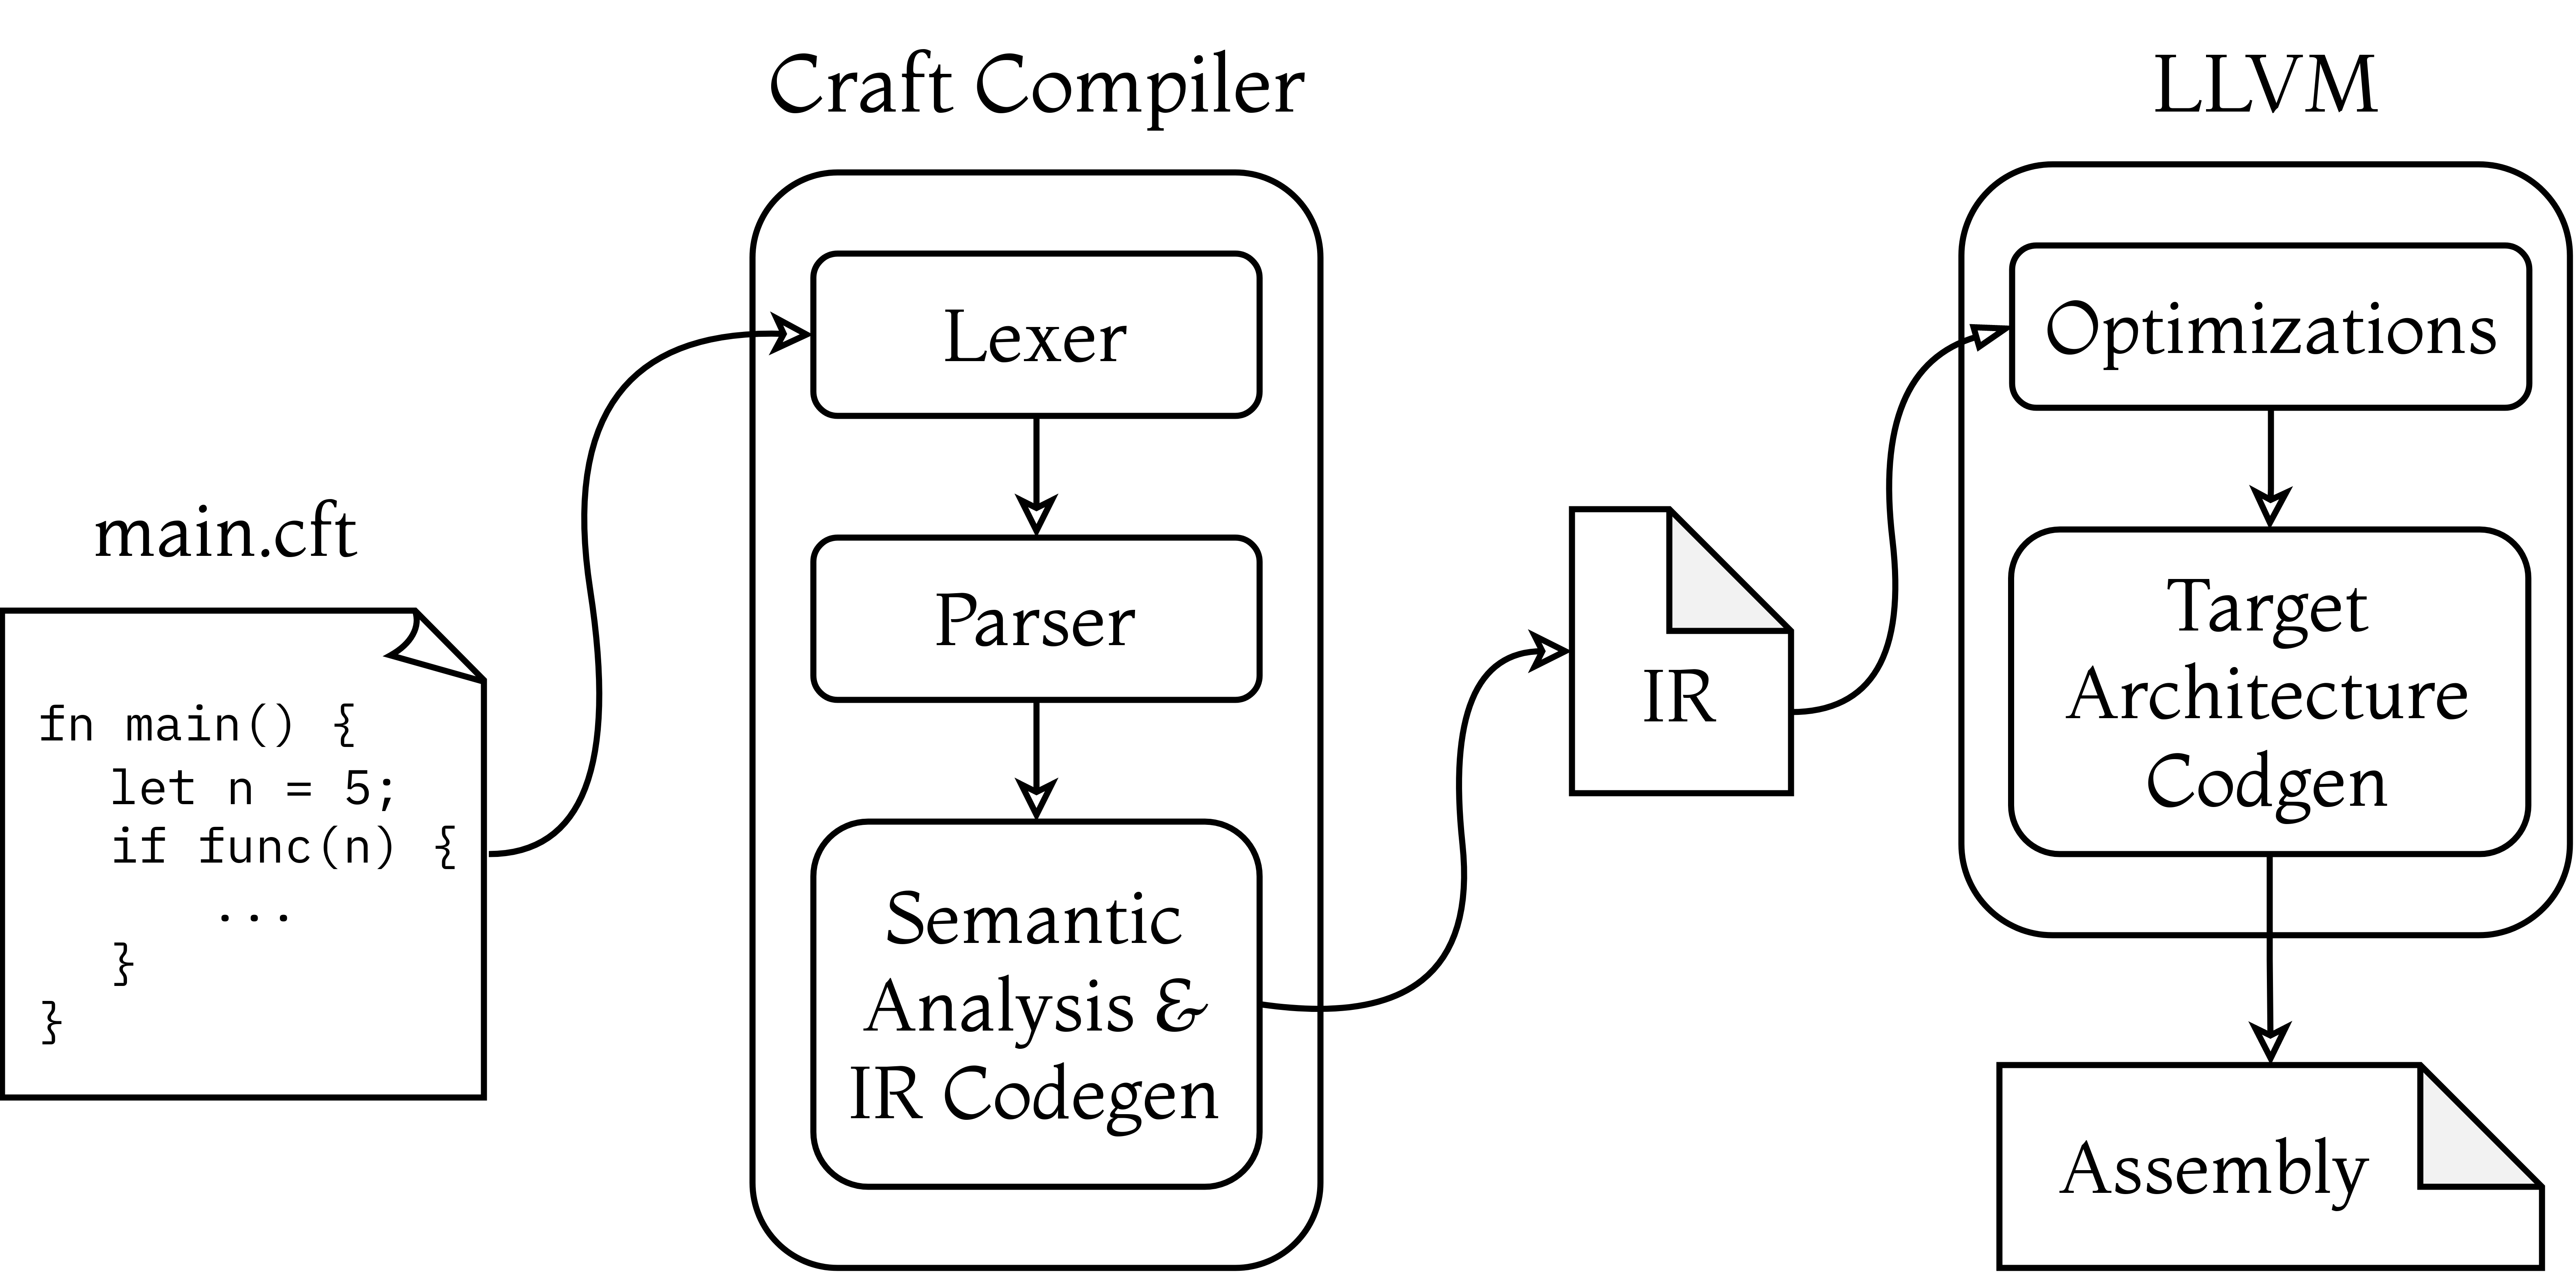
\includegraphics[width=\linewidth]{arch}
\caption{Diagram showing the compilation workflow of a Craft program}
\end{figure}

\subsection{Lexing} 
This step consists of breaking the source code into a sequence of tokens. A
token is a basic building block of the languages, such as a keyword or an
identifier.

A lexer can be implemented rather easily, by using a state machine. An approach
to do it programmatically could be the following:

\begin{enumerate}
    \item Start by reading the source code character by character until we reach
        the end.
    \item If the character by itself forms a valid sequence (e.g. a parenthesis)
        we create a token from it. If it doesn't, we continue reading characters
        until we find a valid sequence. 
\end{enumerate}

Note that sometimes we may find a valid sequence, but that's not enough to
create a token, since it may be the start of another longer and valid sequence.
We may need to check the following character/s to check weather it continues. An
example of such case would be the '\texttt{>}' operator, since, by itself is a
valid sequence, but it may be the start of the '\texttt{>=}' operator. So we
need to check if the next character is an '\texttt{=}' or something else.

The lexer requires a bit of work to set up, but after that, expanding it is 
trivial, since we only need to add a new word to the list of reserved words, in 
the case we want to add a reserved word, or add a new rule that detects a new 
symbol for example.


\subsection{Parsing}
The lexer allowed us to identify the simbols of the program, but it does not 
allow us to determine if their order is correct, or if they follow the rules of
the language (i.e. it's grammatically correct). That is the job of the parser.

The parser takes the sequence of tokens obtained from the lexer and
transforms it into an Abstract Syntax Tree (AST). This tree represents the
structure of the program and determines its syntactic structure. It will tell us
the order in which we need to execute the instruction.

To generate the AST compilers use a context free grammar. A grammar is a set of
rules that tells us how to form valid strings of tokens in a specific language.
They are formed of a set of symbols, which can be divided into terminal and
non-terminal symbols, and a set of production rules that specify how the
non-terminal symbols can be replaced by sequences of terminal and non-terminal
symbols. A context free grammar is a type of grammar that, the rules of the grammar do
not depend on the context in which the symbols appear.

The goal of the parser is to make the program obey the rules of the grammar.

Here's an example of a simple grammar for parsing function prototypes:

\begin{small}
\begin{verbatim}
<proto>   ::= fn <id> "(" <params> ")"
<id>      ::= letter {letter | digit | "_"}
<params>  ::= "("{ <param> {, <param> } }")"
<param>   ::= <id>: <type>
\end{verbatim}
\end{small}

If we were to translate the proto rule to code, it would look something like 
this:

\begin{code}
fn parse_prototype() -> (Prototype, Err) {
    // we expect to find the fn keyword,
    // else it's an error
    match current_token().kind {
        // The advance function moves to the next token
        TokenKind::Fn => advance(),
        _ => return Err("Expected fn keyword"),
    };

    // we expect to find the function name,
    // else it's an error
    let name = match current_token().kind {
        TokenKind::Identifier => current_token().lexeme,
        _ => return Err("Expected an identifier"),
    };

    advance();

    // we call the params rule
    let params = parse_params();

    // we are done, we return a struct 
    // with the info of the prototype
    return Prototype { 
        name,
        params,
    };
}
\end{code}

\subsection{Semantic Analysis and [IR] Code Generation}
Once we have an AST, we can traverse it to generate the LLVM IR. Since this is a
simple compiler, we are going to do the semantic analysis in this step. With 
more complex compilers, we may want to create a specific step of semantic 
analysis, but in out case it is not necessary.

LLVM has the concept of modules. A module contains all the information
associated with one code file. If we have multiple files, we simply have to
create different modules and link them. Modules contain functions and functions
are made up of instructions, similar to the instructions we find in assembly.

Let's see an example of a small piece of code and what it would look like in the
intermediate representation of LLVM. We have the following function that
receives two integers and returns the maximum:

\begin{code}
fn max(int a, int b) int {
    if a > b { a } else { b }
}
\end{code}

If we translate it to LLVM IR we have the following code:

\begin{code}
define i32 @max(i32 %a, i32 %b) {
entry:
  %0 = icmp sgt i32 %a, %b
  br i1 %0, label %btrue, label %bfalse

btrue:
  br label %end

bfalse:
  br label %end

end:
  %retval = phi i32 [%a, %btrue], [%b, %bfalse]
  ret i32 %retval
}
\end{code}

The first line of the previous code defines a function, which receives two
32 bits integers. A label entry is defined below. These tags are like assembly
tags, and we can jump to them.

The first thing it does, on the 'entry' tag, is comparing both integers (i.e.
the if condition). The \texttt{'sgt'} keyword, means 'signed greater than',
which, as the names says, does a greater than signed comparison. The result of
the comparison is a one bit integer which acts like a boolean. If it's true, it
will jump to the label \texttt{btrue}, otherwise to the label \texttt{bfalse}.

In this case the two branches do the same thing: a jump to the label
\texttt{end}. There we come across a concept called phi nodes. The phi nodes
are kind of an inverted if. Depending on where we did the jump we will assign
one value or another to the variable \texttt{retval}. If we come from
\texttt{btrue}, \texttt{retval} is assigned \texttt{\%a}, and if we come from 
\texttt{bfalse} it is assigned to \texttt{\%b}.

Now, why do the two branches jump to the \texttt{end} tag and then do a
conditional again in the \texttt{end} block? Couldn't we assign the value of
\texttt{retval} directly inside the branch \texttt{btrue} or \texttt{bfalse} and
spare us that third conditional? Well the answer is no, because then we would be
generating code that is not in SSA form. And as we mentioned earlier, LLVM
requires the generated code to be in SSA form. And that's why phi nodes exist,
to be able to solve this types of problems.

\subsubsection{LLVM API}

It's important to understand the LLVM IR, but generating all of that code by 
hand is a lot of work and it would require us to put a lot of infrastructure in
place. Fortunately for us, LLVM comes with a C++ API, that makes generating the
IR a lot easier. There's the little problem that we are not using C++, but 
thankfully, there's a Rust library called Inkwell, that offers a comfortable and 
idiomatic Rust interface to the LLVM API. Under the hood it calls the C++ API
by using FFI (Foreign Function Interface).

The API is made of several entities. The most fundamental one is the
\texttt{BasicBlock}, which represents the blocks that we find inside a function,
i.e. the set of instructions we find within a label. If we group a bunch of
BasicBlocks, we have an entity call \texttt{Function}, which, you guess it 
represents a function in the IR. And by grouping a bunch of functions we get the
\texttt{Module} entity. As you may notice these entities represent the different
parts that we saw when we talked about the IR.

Another important entity is \texttt{Context}. We just need and instance of it, 
and it will keep track of the state of the compilation.

Finally we have the \texttt{Builder} entity, which is the one in charge of 
actually generating the code. For example, if we want to generate a comparison,
like the one we saw on the IR example, we would call the \texttt{Builder}, 
telling it which instruction to generate:

\texttt{Builder.CreateICmpSGT(a, b, "some-name")}

The first two parameters are the two values being compared. The third 
indicates the name of the generated variable (we can give it any name we want,
it's only useful for debugging).

The previous call will generate the following code (which is the third line of
the IR example we saw):

\texttt{\%nom = icmp sgt i32 \%a, \%b}

\section{Results}
\texttt{TODO: Benchamarks}

\section{Conclusions}
\texttt{TODO}

\begin{thebibliography}{11}

\bibitem{llvmtut} \textit{LLVM Kaleidoscope Tutorial: Implementing a Language with LLVM}. Accessed the 25th of October 2022, from \url{https://llvm.org/docs/tutorial}
\bibitem{llvm4plc} Rathi, M. \textit{A complete guide to LLVM for programming language creators}. Mukuls Blogs. Accessed the 2nd of November 2022, from \\\url{https://mukulrathi.com/create-your-own-programming-language/llvm-ir-cpp-api-tutorial}
\bibitem{ci} Nystrom, R. \textit{Crafting Interpreters}. Published July 2021. ISBN 0990582930.
\bibitem{mhlctllvm} \textit{Mapping High Level Constructs to LLVM IR}. Accessed the 20th of October 2022 from \\\url{https://mapping-high-level-constructs-to-llvm-ir.readthedocs.io/en/latest/README.html}
\bibitem{inkwell} \textit{Inkwell Documentation}. Accessed the 4th of October 2022 from \\\url{https://thedan64.github.io/inkwell/inkwell/index.html}
\bibitem{compilergo} Ball, T. \textit{Writing A Compiler In Go}. Published August 2018. ISBN 398201610X.

\end{thebibliography}

\appendix

\section*{Apèndix}

\begin{code}
struct ComplexNumber {
    real:      f64
    imaginary: f64
}

fn add(x: ComplexNumber, y: ComplexNumber) ComplexNumber {
    ComplexNumber!{
        real: x.real + y.real,
        imaginary: x.imaginary + y.imaginary,
    }
}

fn multiply(x: ComplexNumber, y: ComplexNumber) ComplexNumber {
    ComplexNumber!{
        real: x.real * y.real - x.imaginary * y.imaginary,
        imaginary: x.real * y.imaginary + x.imaginary * y.real,
    }
}

fn main() {
    let x = ComplexNumber!{
        real: 1.0,
        imaginary: 2.0,
    };
    let y = ComplexNumber!{
        real: 3.0,
        imaginary: 4.0,
    };

    let z = add(x, y);
    printf("The sum of x and y is %f + %fi\n", z.real, z.imaginary);

    z = multiply(x, y);
    printf("The product of x and y is %f + %fi\n", z.real, z.imaginary);
}
\end{code}

\setcounter{section}{1}

\subsection{Secció d'Apèndix}
.... ... ..... ... ..... ... ... ..... .... .

\subsection{Secció d'Apèndix}
.... ... ..... ... ..... ... ... ..... .... .

\end{document}
